\subsection{Das ,,fertige`` Produkt}\label{ku_produkt}
\begin{figure}[H]
	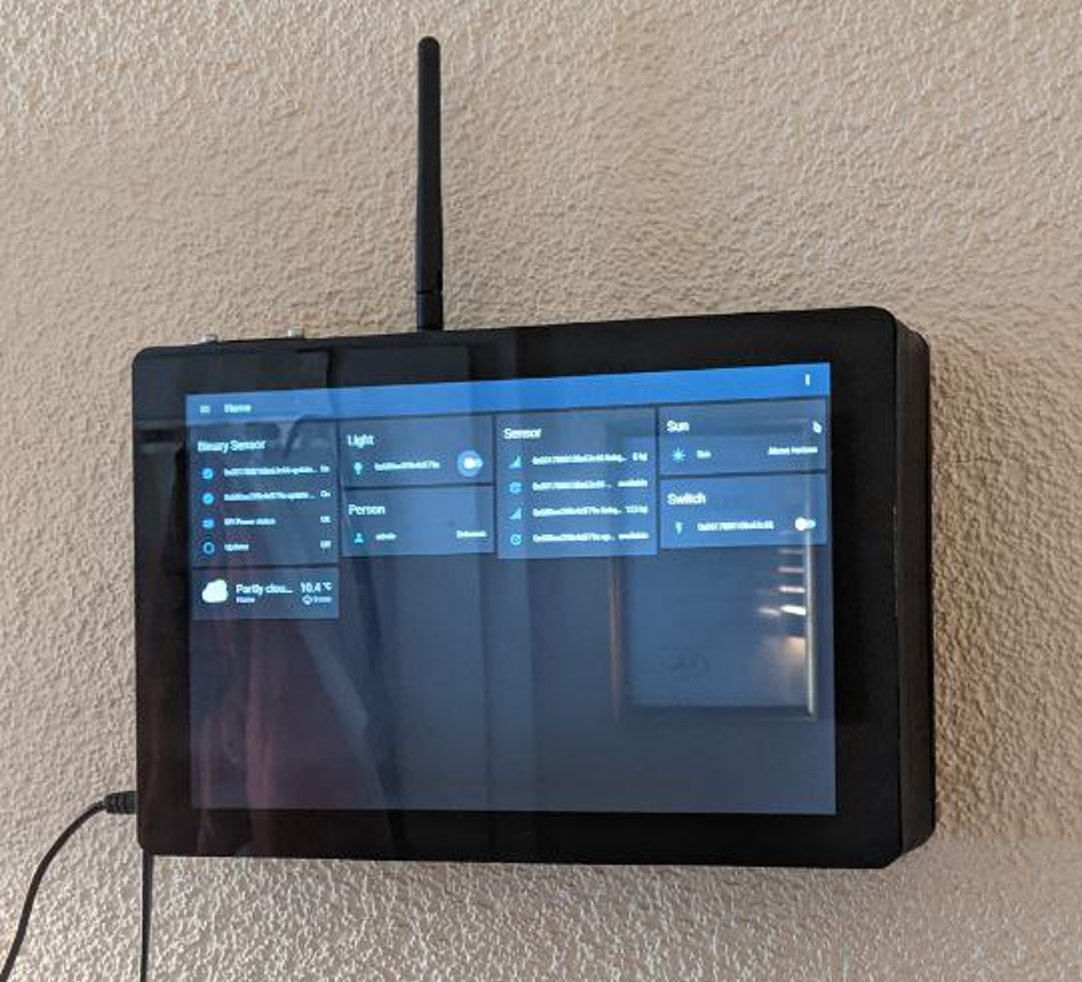
\includegraphics[width=1\textwidth]{img/fertiges_geraet.png}
	\caption[Smart Home Zentrale]{Smart Home Zentrale}
	\label{fig:smart-home-zentrale}
\end{figure}
\noindent In Abbildung \ref{fig:smart-home-zentrale} wird das Ergebnis der Technikerarbeit von Felix Kuschel und Manuel Starz präsentiert. 
Die Smart Home Zentrale verfügt über eine ZigBee-Antenne, einem 10.1'' großen Touchbildschirm und der Möglichkeit, per LAN und oder WLAN mit dem Heimnetz in Verbindung zu treten.\par
\noindent Das Gehäuse ist für die Wand-Montage (vgl. Abb. \ref{fig:smart-home-zentrale}: \nameref{fig:smart-home-zentrale}) oder als Aufstellgerät (vgl. Abb. \ref{fig:case-with-feet}: \nameref{fig:case-with-feet}) entworfen worden.
\begin{figure}[H]
	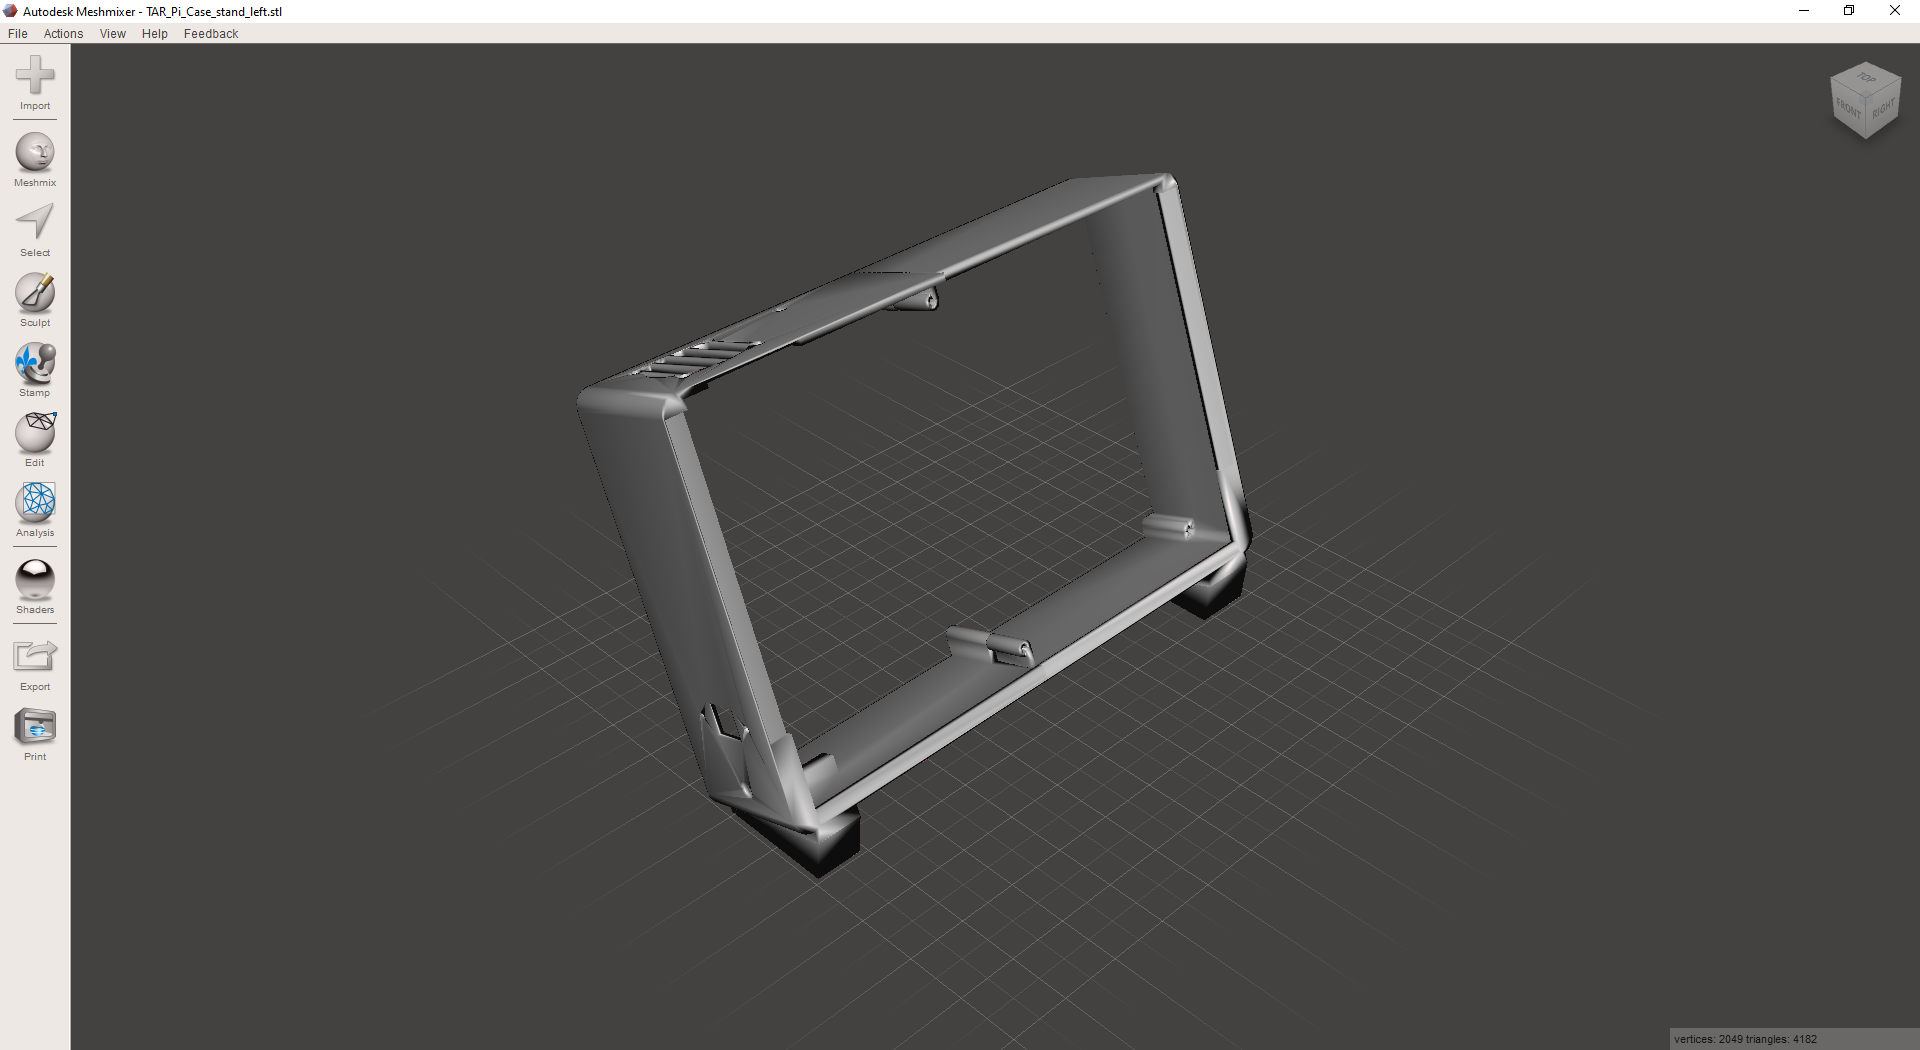
\includegraphics[width=1\textwidth]{img/stand_case.png}
	\caption[Gehäuse mit Füßen (Render in Meshmixer)]{Gehäuse mit Füßen (Render in Meshmixer)}
	\label{fig:case-with-feet}
\end{figure}